\documentclass[12pt]{scrartcl}
\usepackage[hagavi]{azzam}
\usetikzlibrary{calc,angles}
\renewcommand{\qedsymbol}{$\blacksquare$}

% Geometri Pembuktian Dasar - Modul (gabungan Materi dan Soal Latihan)
% Level pembuktian awal: angle chasing, kekongruenan, kesebangunan, segiempat siklik.
% 12 soal latihan PEMBUKTIAN (esai/uraian): 4 kelompok teknik,
% tiap kelompok urut mudah, sedang, sukar.
% Sumber soal: berkas osp-sma-categorized.tex, osn-sma-categorized.tex,
% dan emc-2020-junior.tex di arsip Project-Helvethia.
% _Ujian tetap terpisah. Berkas _Solusi yang ada membahas set soal isian
% lama dan belum diperbarui mengikuti set pembuktian ini.
% Sumber tiap soal latihan dimunculkan di PDF sebagai \item (Sumber);
% komentar menyimpan detail lengkap.

\title{Geometri Pembuktian Dasar - Modul}
\date{13 November 2026}

\begin{document}
\maketitle

\renewcommand*\contentsname{Daftar Isi}
\tableofcontents

\newpage

Modul ini melatih langkah awal menulis bukti geometri. Isinya empat teknik
dasar: kejar sudut, kekongruenan, kesebangunan, dan segiempat talibusur.
Tiap teknik disertai ciri yang membantu mengenalinya di soal, lalu contoh
yang dikerjakan tuntas. Soal latihan di bagian akhir tersusun dari mudah
ke sukar di tiap kelompok.

\part*{Materi}

\section{Angle Chasing}

Teknik pertama adalah \istilah{kejar sudut}{angle chasing}. Intinya
sederhana. Tulis semua sudut yang diketahui, lalu kejar sisanya memakai
kesamaan sudut yang tersedia.

\begin{fact}[Sudut segitiga dan garis sejajar]
Dalam segitiga $ABC$ berlaku
\[ \angle A + \angle B + \angle C = 180^\circ. \]
Dua sudut yang berpelurus berjumlah $180^\circ$.
Dua \istilah{sudut bertolak belakang}{vertical angles} sama besar.
Jika dua garis sejajar dipotong oleh garis lain, pasangan
\istilah{sudut sehadap}{corresponding angles} yang terbentuk sama besar.
\end{fact}

\begin{example}
Pada segitiga $ABC$, \istilah{garis bagi}{angle bisector} sudut $A$ dan
sudut $B$ berpotongan di $I$. Buktikan
\[ \angle AIB = 90^\circ + \frac{\angle C}{2}. \]
\begin{center}
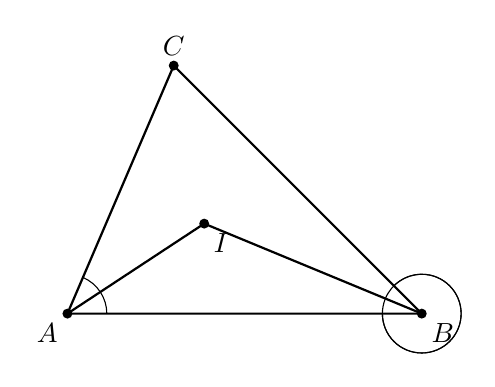
\begin{tikzpicture}[scale=0.9]
    \coordinate (A) at (0,0);
    \coordinate (B) at (5,0);
    \coordinate (C) at (1.5,3.5);
    \coordinate (I) at (1.93,1.27);
    \draw[thick] (A) -- (B) -- (C) -- cycle;
    \draw[thick] (A) -- (I);
    \draw[thick] (B) -- (I);
    \pic [draw, angle radius=5mm] {angle = B--A--I};
    \pic [draw, angle radius=5mm] {angle = I--A--C};
    \pic [draw, angle radius=5mm] {angle = A--B--I};
    \pic [draw, angle radius=5mm] {angle = I--B--C};
    \fill (A) circle (2pt);
    \fill (B) circle (2pt);
    \fill (C) circle (2pt);
    \fill (I) circle (2pt);
    \node[below left] at (A) {$A$};
    \node[below right] at (B) {$B$};
    \node[above] at (C) {$C$};
    \node[below right] at (I) {$I$};
\end{tikzpicture}
\end{center}
\end{example}
\begin{proof}[Solusi]
Tulis sudut di $I$ memakai jumlah sudut segitiga $ABI$:
\begin{align*}
\angle AIB &= 180^\circ - \angle BAI - \angle ABI \\
&= 180^\circ - \frac{\angle A}{2} - \frac{\angle B}{2} \\
&= 180^\circ - \frac{\angle A + \angle B}{2}.
\end{align*}
Karena $\angle A + \angle B = 180^\circ - \angle C$:
\begin{align*}
\angle AIB &= 180^\circ - \frac{180^\circ - \angle C}{2} \\
&= 90^\circ + \frac{\angle C}{2}.
\end{align*}
\end{proof}

\begin{fact}[Segitiga sama kaki]
\istilah{Segitiga sama kaki}{isosceles triangle} memiliki sepasang sisi
sama panjang. Sisi yang sama panjang menghadap sudut yang sama besar,
dan sebaliknya: sudut yang sama besar dihadap oleh sisi yang sama panjang.
\end{fact}

\begin{example}
Diberikan segitiga $ABC$ sama kaki dengan $AB = AC$ dan
$\angle BAC = 36^\circ$. Titik $D$ pada sisi $AC$ memenuhi
$\angle DBC = 36^\circ$. Buktikan $AD = BD$.
\begin{center}
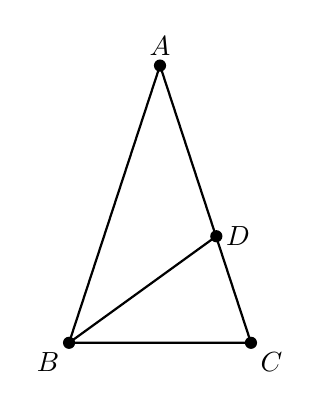
\begin{tikzpicture}[scale=1.1]
    \coordinate (A) at (0,3.2);
    \coordinate (B) at (-1.05,0);
    \coordinate (C) at (1.05,0);
    \coordinate (D) at (0.65,1.23);
    \draw[thick] (A) -- (B) -- (C) -- cycle;
    \draw[thick] (B) -- (D);
    \fill (A) circle (2pt);
    \fill (B) circle (2pt);
    \fill (C) circle (2pt);
    \fill (D) circle (2pt);
    \node[above] at (A) {$A$};
    \node[below left] at (B) {$B$};
    \node[below right] at (C) {$C$};
    \node[right] at (D) {$D$};
\end{tikzpicture}
\end{center}
\end{example}
\begin{proof}[Solusi]
Karena $AB = AC$, sudut alasnya sama:
\begin{align*}
\angle ABC &= \angle ACB \\
&= \frac{180^\circ - 36^\circ}{2} \\
&= 72^\circ.
\end{align*}
Sudut $ABD$ sisanya:
\begin{align*}
\angle ABD &= \angle ABC - \angle DBC \\
&= 72^\circ - 36^\circ \\
&= 36^\circ.
\end{align*}
Jadi $\angle ABD = \angle BAD = 36^\circ$. Segitiga $ABD$ sama kaki
dengan $AD = BD$.
\end{proof}

\begin{fact}[Sudut luar]
\istilah{Sudut luar}{exterior angle} segitiga sama dengan jumlah dua sudut
dalam yang tidak bersisian dengannya. Pada segitiga $ABC$ dengan $D$ pada
perpanjangan $BC$:
\[ \angle ACD = \angle A + \angle B. \]
\end{fact}

\begin{example}
Diberikan segitiga $ABC$ sama kaki dengan $AB = AC$. Titik $D$ pada
perpanjangan $BA$ dengan $A$ di antara $B$ dan $D$. Buktikan
$\angle DAC = 2\angle ABC$.
\begin{center}
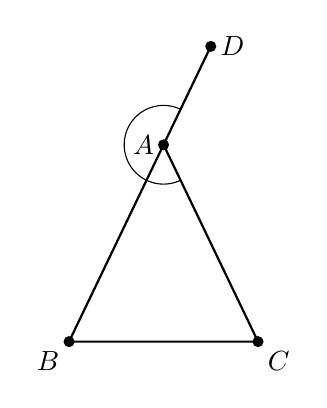
\begin{tikzpicture}[scale=1.0]
    \coordinate (A) at (0,2.5);
    \coordinate (B) at (-1.2,0);
    \coordinate (C) at (1.2,0);
    \coordinate (D) at (0.6,3.75);
    \draw[thick] (A) -- (B) -- (C) -- cycle;
    \draw[thick] (A) -- (D);
    \pic [draw, angle radius=5mm] {angle = D--A--C};
    \fill (A) circle (2pt);
    \fill (B) circle (2pt);
    \fill (C) circle (2pt);
    \fill (D) circle (2pt);
    \node[left] at (A) {$A$};
    \node[below left] at (B) {$B$};
    \node[below right] at (C) {$C$};
    \node[right] at (D) {$D$};
\end{tikzpicture}
\end{center}
\end{example}
\begin{proof}[Solusi]
Sudut $DAC$ dan $BAC$ berpelurus:
\[ \angle DAC = 180^\circ - \angle BAC. \]
Karena $AB = AC$, sudut alasnya sama dan
\begin{align*}
\angle BAC &= 180^\circ - \angle ABC - \angle ACB \\
&= 180^\circ - 2\angle ABC.
\end{align*}
Substitusikan:
\begin{align*}
\angle DAC &= 180^\circ - (180^\circ - 2\angle ABC) \\
&= 2\angle ABC.
\end{align*}
\end{proof}

\begin{remark}[Ciri angle chasing]
Angle chasing bekerja saat banyak sudut sudah diketahui. Cari segitiga
sama kaki dan garis yang sejajar. Keduanya memberi kesamaan sudut tanpa
hitungan tambahan.
\end{remark}

\section{Kekongruenan}

Dua segitiga disebut \istilah{kongruen}{congruent} apabila sisi dan sudut
yang bersesuaian sama besar. Sekali kekongruenan terbukti, semua pasangan
sisi dan sudut boleh saling menggantikan.

\begin{fact}[Kriteria kekongruenan]
Dua segitiga kongruen jika memenuhi salah satu kondisi berikut.
\begin{enumerate}
    \item Ketiga sisi yang bersesuaian sama panjang (SSS).
    \item Dua sisi dan sudut apitnya sama besar (SAS).
    \item Dua sudut dan sisi di antaranya sama besar (ASA).
    \item Dua sudut dan satu sisi di luar apitnya sama besar (AAS).
\end{enumerate}
\end{fact}

\begin{example}
Diberikan persegi $ABCD$. Titik $E$ pada sisi $AB$ dan titik $F$ pada sisi
$BC$ memenuhi $AE = BF$. Buktikan $DE = CF$.
\begin{center}
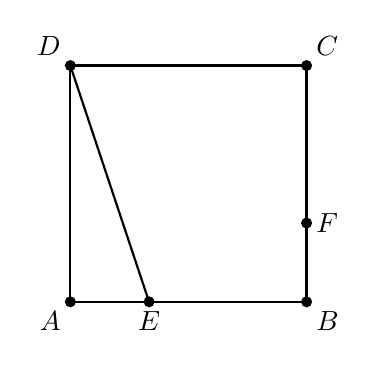
\begin{tikzpicture}[scale=1.0]
    \coordinate (A) at (0,0);
    \coordinate (B) at (3,0);
    \coordinate (C) at (3,3);
    \coordinate (D) at (0,3);
    \coordinate (E) at (1,0);
    \coordinate (F) at (3,1);
    \draw[thick] (A) -- (B) -- (C) -- (D) -- cycle;
    \draw[thick] (D) -- (E);
    \draw[thick] (C) -- (F);
    \fill (A) circle (2pt);
    \fill (B) circle (2pt);
    \fill (C) circle (2pt);
    \fill (D) circle (2pt);
    \fill (E) circle (2pt);
    \fill (F) circle (2pt);
    \node[below left] at (A) {$A$};
    \node[below right] at (B) {$B$};
    \node[above right] at (C) {$C$};
    \node[above left] at (D) {$D$};
    \node[below] at (E) {$E$};
    \node[right] at (F) {$F$};
\end{tikzpicture}
\end{center}
\end{example}
\begin{proof}[Solusi]
Kedua sudut $DAE$ dan $CBF$ siku-siku. Bandingkan segitiga $DAE$ dan
$CBF$:
\begin{align*}
DA &= CB, \\
\angle DAE &= \angle CBF, \\
AE &= BF.
\end{align*}
Baris pertama memakai sisi persegi, baris ketiga memakai yang diketahui.
Jadi $\triangle DAE \cong \triangle CBF$ menurut SAS. Sisi
bersesuaiannya sama: $DE = CF$.
\end{proof}

\begin{fact}[Titik pada garis bagi]
Titik pada garis bagi sudut berjarak sama ke kedua kaki sudut.
\end{fact}

\begin{example}
Garis bagi sudut $A$ pada segitiga $ABC$ memotong $BC$ di $D$. Titik $E$
dan $F$ berturut-turut kaki dari $D$ ke garis $AB$ dan $AC$. Buktikan
$DE = DF$.
\begin{center}
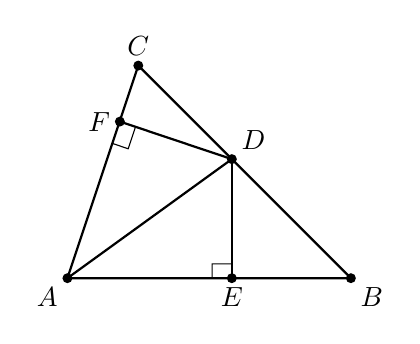
\begin{tikzpicture}[scale=0.9]
    \coordinate (A) at (0,0);
    \coordinate (B) at (4,0);
    \coordinate (C) at (1,3);
    \coordinate (D) at (2.32,1.68);
    \coordinate (E) at (2.32,0);
    \coordinate (F) at (0.74,2.21);
    \draw[thick] (A) -- (B) -- (C) -- cycle;
    \draw[thick] (A) -- (D);
    \draw[thick] (D) -- (E);
    \draw[thick] (D) -- (F);
    \coordinate (tE) at ($(E)!0.12!(D)$);
    \coordinate (tEA) at ($(E)!0.12!(A)$);
    \draw (tE) -- ($(tE)+(tEA)-(E)$) -- (tEA);
    \coordinate (tF) at ($(F)!0.14!(D)$);
    \coordinate (tFA) at ($(F)!0.14!(A)$);
    \draw (tF) -- ($(tF)+(tFA)-(F)$) -- (tFA);
    \fill (A) circle (2pt);
    \fill (B) circle (2pt);
    \fill (C) circle (2pt);
    \fill (D) circle (2pt);
    \fill (E) circle (2pt);
    \fill (F) circle (2pt);
    \node[below left] at (A) {$A$};
    \node[below right] at (B) {$B$};
    \node[above] at (C) {$C$};
    \node[above right] at (D) {$D$};
    \node[below] at (E) {$E$};
    \node[left] at (F) {$F$};
\end{tikzpicture}
\end{center}
\end{example}
\begin{proof}[Solusi]
Segitiga $AED$ dan $AFD$ siku-siku di $E$ dan $F$. Keduanya memenuhi
\begin{align*}
\angle EAD &= \angle FAD, \\
AD &= AD.
\end{align*}
Dua sudut dan sisi miringnya sama, jadi $\triangle AED \cong \triangle
AFD$ menurut AAS. Sisi bersesuaiannya sama: $DE = DF$.
\end{proof}

\begin{remark}[Ciri kekongruenan]
Kongruen cocok saat soal memberi ruas sama panjang atau meminta membuktikan
dua ruas sama. Cari pasangan segitiga yang memuat ruas itu. Cocokkan sisi
dan sudut apitnya.
\end{remark}

\section{Kesebangunan}

Dua segitiga \istilah{sebangun}{similar} apabila sudut yang bersesuaian
sama besar. Sisi yang bersesuaiannya lalu sebanding, dan faktor
perbandingannya sama untuk ketiga pasangan sisi.

\begin{fact}[Kriteria kesebangunan]
Dua segitiga sebangun jika memenuhi salah satu kondisi berikut.
\begin{enumerate}
    \item Dua sudut yang bersesuaian sama besar (AA).
    \item Dua pasang sisi sebanding dan sudut apitnya sama besar (SAS).
    \item Ketiga pasang sisi sebanding (SSS).
\end{enumerate}
Kriteria AA yang paling sering dipakai. Dua sudut sama memaksa sudut
ketiga sama, karena jumlahnya $180^\circ$.
\end{fact}

\begin{example}
Titik $D$ dan $E$ berturut-turut pada sisi $AB$ dan $AC$ dari segitiga
$ABC$ sehingga $DE \parallel BC$. Buktikan
\[ \frac{AD}{AB} = \frac{AE}{AC} = \frac{DE}{BC}. \]
\begin{center}
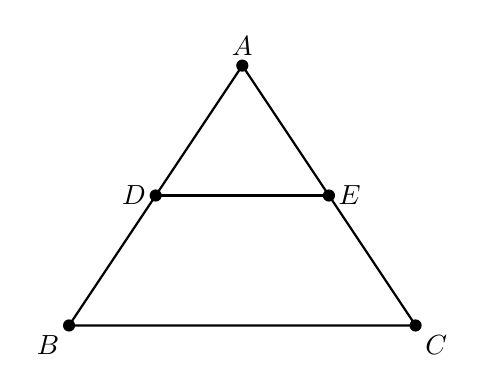
\begin{tikzpicture}[scale=1.1]
    \coordinate (A) at (0,3);
    \coordinate (B) at (-2,0);
    \coordinate (C) at (2,0);
    \coordinate (D) at (-1,1.5);
    \coordinate (E) at (1,1.5);
    \draw[thick] (A) -- (B) -- (C) -- cycle;
    \draw[thick] (D) -- (E);
    \fill (A) circle (2pt);
    \fill (B) circle (2pt);
    \fill (C) circle (2pt);
    \fill (D) circle (2pt);
    \fill (E) circle (2pt);
    \node[above] at (A) {$A$};
    \node[below left] at (B) {$B$};
    \node[below right] at (C) {$C$};
    \node[left] at (D) {$D$};
    \node[right] at (E) {$E$};
\end{tikzpicture}
\end{center}
\end{example}
\begin{proof}[Solusi]
Karena $DE \parallel BC$, sudut sehadapnya sama:
\begin{align*}
\angle ADE &= \angle ABC, \\
\angle AED &= \angle ACB.
\end{align*}
Jadi $\triangle ADE \sim \triangle ABC$ menurut AA. Sisi
bersesuaiannya sebanding:
\[ \frac{AD}{AB} = \frac{AE}{AC} = \frac{DE}{BC}. \]
\end{proof}

\begin{theorem}[Garis bagi sudut]
Garis bagi sudut $A$ pada segitiga $ABC$ memotong $BC$ di $D$. Maka
\[ \frac{BD}{DC} = \frac{AB}{AC}. \]
\end{theorem}

\begin{example}
Buktikan teorema garis bagi sudut di atas.
\begin{center}
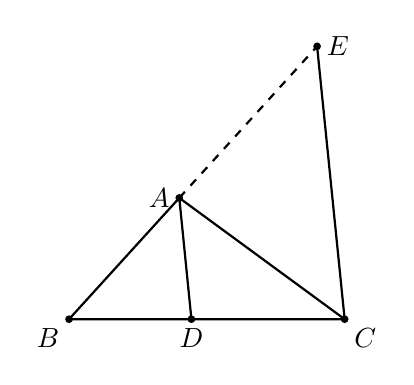
\begin{tikzpicture}[scale=0.7]
    \coordinate (A) at (2,2.2);
    \coordinate (B) at (0,0);
    \coordinate (C) at (5,0);
    \coordinate (D) at (2.22,0);
    \coordinate (E) at (4.5,4.95);
    \draw[thick] (A) -- (B) -- (C) -- cycle;
    \draw[thick] (A) -- (D);
    \draw[thick] (C) -- (E);
    \draw[thick,dashed] (A) -- (E);
    \fill (A) circle (2pt);
    \fill (B) circle (2pt);
    \fill (C) circle (2pt);
    \fill (D) circle (2pt);
    \fill (E) circle (2pt);
    \node[left] at (A) {$A$};
    \node[below left] at (B) {$B$};
    \node[below right] at (C) {$C$};
    \node[below] at (D) {$D$};
    \node[right] at (E) {$E$};
\end{tikzpicture}
\end{center}
\end{example}
\begin{proof}[Solusi]
Tarik garis melalui $C$ yang sejajar $AD$. Garis ini memotong perpanjangan
$BA$ di $E$. Karena $AD \parallel EC$:
\begin{align*}
\angle BAD &= \angle BEC, \\
\angle DAC &= \angle ACE.
\end{align*}
Baris pertama memakai sudut sehadap, baris kedua memakai sudut
berseberangan. Karena $AD$ garis bagi, $\angle BAD = \angle DAC$.
Jadi $\angle BEC = \angle ACE$. Segitiga $ACE$ sama kaki dengan
$AE = AC$.

Pada segitiga $BEC$, ruas $AD$ sejajar $EC$. Menurut contoh sebelumnya,
sisi-sisinya terbagi proporsional:
\begin{align*}
\frac{BD}{DC} &= \frac{BA}{AE} \\
&= \frac{AB}{AC}.
\end{align*}
\end{proof}

\begin{remark}[Ciri kesebangunan]
Kesebangunan muncul bersama garis sejajar dan perbandingan panjang. Cari
dua sudut yang sama. Pasangan sisi di depan sudut sama itu yang sebanding.
\end{remark}

\section{Segiempat Siklik}

Empat titik yang terletak pada satu lingkaran membentuk
\istilah{segiempat talibusur}{cyclic quadrilateral}. Lingkaran yang
melaluinya disebut \istilah{lingkaran luar}{circumcircle}. Selanjutnya
segiempat seperti itu disebut siklik.

\begin{theorem}[Kriteria siklik]
Segiempat $ABCD$ siklik jika memenuhi salah satu kondisi berikut.
\begin{enumerate}
    \item Jumlah dua sudut berhadapan sama dengan $180^\circ$.
    \item Dua sudut yang menghadap ruas garis yang sama besarnya sama.
\end{enumerate}
\end{theorem}

\begin{example}
Titik $D$ dan $E$ berturut-turut pada sisi $AB$ dan $AC$ dari segitiga
$ABC$ sehingga $\angle AED = \angle ABC$. Buktikan $B$, $C$, $E$, $D$
siklik.
\begin{center}
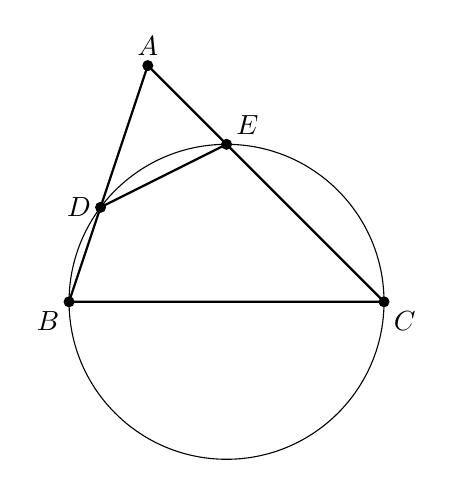
\begin{tikzpicture}[scale=1.0]
    \coordinate (A) at (1,3);
    \coordinate (B) at (0,0);
    \coordinate (C) at (4,0);
    \coordinate (D) at (0.4,1.2);
    \coordinate (E) at (2,2);
    \draw[thick] (A) -- (B) -- (C) -- cycle;
    \draw[thick] (D) -- (E);
    \draw[thin] (2,0) circle (2);
    \fill (A) circle (2pt);
    \fill (B) circle (2pt);
    \fill (C) circle (2pt);
    \fill (D) circle (2pt);
    \fill (E) circle (2pt);
    \node[above] at (A) {$A$};
    \node[below left] at (B) {$B$};
    \node[below right] at (C) {$C$};
    \node[left] at (D) {$D$};
    \node[above right] at (E) {$E$};
\end{tikzpicture}
\end{center}
\end{example}
\begin{proof}[Solusi]
Sudut $AED$ dan $DEC$ berpelurus:
\begin{align*}
\angle DEC &= 180^\circ - \angle AED \\
&= 180^\circ - \angle ABC.
\end{align*}
Jadi
\[ \angle DEC + \angle DBC = 180^\circ. \]
Dua sudut berhadapan segiempat $BCED$ berjumlah $180^\circ$. Segiempat
itu siklik.
\end{proof}

\begin{fact}[Thales]
Sudut yang menghadap diameter lingkaran siku-siku. Jika $AB$ diameter
dan $C$ titik pada lingkaran selain $A$ dan $B$, maka
$\angle ACB = 90^\circ$.
\end{fact}

\begin{example}
Buktikan teorema Thales di atas.
\begin{center}
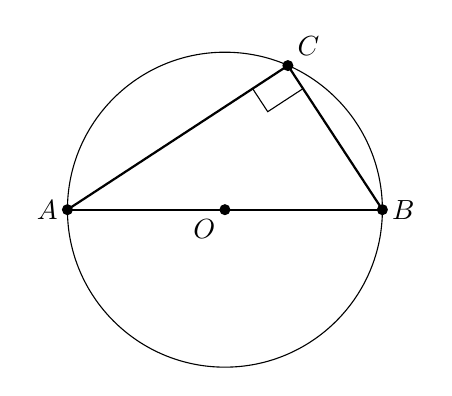
\begin{tikzpicture}[scale=1.0]
    \coordinate (O) at (0,0);
    \coordinate (A) at (-2,0);
    \coordinate (B) at (2,0);
    \coordinate (C) at (0.8,1.83);
    \draw[thin] (O) circle (2);
    \draw[thick] (A) -- (B);
    \draw[thick] (A) -- (C) -- (B);
    \coordinate (tC) at ($(C)!0.16!(A)$);
    \coordinate (tCB) at ($(C)!0.16!(B)$);
    \draw (tC) -- ($(tC)+(tCB)-(C)$) -- (tCB);
    \fill (O) circle (2pt);
    \fill (A) circle (2pt);
    \fill (B) circle (2pt);
    \fill (C) circle (2pt);
    \node[below left] at (O) {$O$};
    \node[left] at (A) {$A$};
    \node[right] at (B) {$B$};
    \node[above right] at (C) {$C$};
\end{tikzpicture}
\end{center}
\end{example}
\begin{proof}[Solusi]
Misalkan $O$ titik tengah $AB$. Maka $OA = OB = OC$ sebagai jari-jari.
Kedua segitiga $OAC$ dan $OBC$ sama kaki. Tulis
$\angle OAC = \angle OCA = \alpha$ dan
$\angle OBC = \angle OCB = \beta$. Jumlah sudut segitiga $ABC$:
\begin{align*}
2\alpha + 2\beta &= 180^\circ, \\
\alpha + \beta &= 90^\circ.
\end{align*}
Padahal $\angle ACB = \alpha + \beta$. Jadi $\angle ACB = 90^\circ$.
\end{proof}

\begin{remark}[Ciri segiempat siklik]
Segiempat siklik patut dicurigai saat dua sudut siku menghadap ruas yang
sama. Ciri lain: dua sudut sama menghadap ruas yang sama. Sekali siklik
terbukti, kejar sudut dapat pindah ke busur lain.
\end{remark}

\part*{Soal Latihan}

\section{Angle Chasing}

\begin{enumerate}

	% Source: OSN SMA 2007 No. 1 (Esai)
	% Jawaban: Terbukti
	\item (OSN 2007)
	Misalkan $ABC$ segitiga dengan $\angle ABC=\angle ACB=70^{\circ}$. Misalkan titik $D$ pada sisi $BC$ sehingga $AD$ garis tinggi, titik $E$ pada sisi $AB$ sehingga $\angle ACE=10^{\circ}$, dan titik $F$ adalah perpotongan $AD$ dan $CE$. Buktikan bahwa $CF=BC.$

	% Source: OSP SMA 2015 No. 3 (Esai)
	% Jawaban: Terbukti
	\item (OSP 2015)
	Diberikan segitiga samakaki $ABC$, dengan $AB=AC$. Misalkan $D$ titik pada segmen $BC$ sehingga $BD=2DC$. Misalkan pula bahwa $P$ titik pada segmen $AD$ sehingga $\angle BAC=\angle BPD$. Buktikan bahwa $\angle BAC=2\angle DPC$.

	% Source: OSP SMA 2018 No. 3 (Esai)
	% Jawaban: Terbukti
	\item (OSP 2018)
	Misalkan $\Gamma_1$ dan $\Gamma_2$ lingkaran berbeda dengan panjang jari-jari sama dan berturut-turut berpusat di titik $O_1$ dan $O_2$. Lingkaran $\Gamma_1$ dan $\Gamma_2$ bersinggungan di titik $P$. Garis $\ell$ melalui $O_1$ menyinggung $\Gamma_2$ di titik $A$. Garis $\ell$ memotong $\Gamma_1$ di titik $X$ dengan $X$ di antara $A$ dan $O_1$. Misalkan $M$ titik tengah $AX$ dan $Y$ titik potong $PM$ dengan $\Gamma_2$ dengan $Y \neq P$. Buktikan bahwa $XY$ sejajar $O_1O_2$.

\end{enumerate}

\section{Kekongruenan}

\begin{enumerate}[resume]

	% Source: OSP SMA 2007 No. 1 (Esai)
	% Jawaban: Terbukti
	\item (OSP 2007)
	Misalkan $ABCD$ sebuah segiempat dengan $AB=BC=CD=DA$.
	\begin{enumerate}
	    \item Buktikan bahwa titik $A$ harus berada di luar segitiga $BCD$.
	    \item Buktikan bahwa setiap pasangan sisi berhadapan pada $ABCD$ selalu sejajar.
	\end{enumerate}

	% Source: OSP SMA 2024 No. 3 (Uraian)
	% Jawaban: Terbukti
	\item (OSP 2024)
	Pada segitiga $ABC$, titik $X, Y$, dan $Z$ masing-masing merupakan titik tengah dari $BC, CA$, dan $AB$ berturut-turut. Garis sumbu $AB$ memotong garis $XY$ dan garis $AC$ berturut-turut pada $Z_1$ dan $Z_2$. Garis sumbu $AC$ memotong garis $XZ$ dan garis $AB$ berturut-turut pada $Y_1$ dan $Y_2$. Misalkan $K$ adalah titik sehingga $KZ_1=KZ_2$ dan $KY_1=KY_2$. Buktikan bahwa $KB=KC$.

	% Source: OSP SMA 2021 No. 8 (Esai)
	% Jawaban: Terbukti
	\item (OSP 2021)
	Diberikan segitiga $ABC$ dengan titik berat $G$. Titik $D$ merupakan titik tengah $AC$. Garis yang melalui $G$ dan sejajar dengan $BC$ memotong $AB$ di $E$. Buktikan bahwa $\angle AEC=\angle DGC$ jika dan hanya jika $\angle ACB=90^\circ$.

\end{enumerate}

\section{Kesebangunan}

\begin{enumerate}[resume]

	% Source: OSP SMA 2006 No. 1 (Esai)
	% Jawaban: Terbukti
	\item (OSP 2006)
	Misalkan segitiga $ABC$ siku-siku di $B$. Garis tinggi dari $B$ memotong sisi $AC$ di titik $D$. Jika titik $E$ dan $F$ berturut-turut adalah titik tengah $BD$ dan $CD$, buktikan bahwa $AE \perp BF$.

	% Source: OSP SMA 2008 No. 3 (Esai; huruf titik dimath-mode-kan, $$ diganti \[ \])
	% Jawaban: Terbukti
	\item (OSP 2008)
	Lingkaran dalam dari segitiga $ABC$, menyinggung sisi-sisi $BC$, $CA$, dan $AB$ berturut-turut di $D$, $E$, dan $F$. Melalui $D$, ditarik garis tegak lurus $EF$ yang memotong $EF$ di $G$. Buktikan bahwa
	\[ \frac{FG}{EG}=\frac{BF}{CE}. \]

	% Source: OSP SMA 2014 No. 4 (Esai)
	% Jawaban: Terbukti
	\item (OSP 2014)
	Misalkan $\Gamma$ adalah lingkaran luar segitiga $ABC$. Satu lingkaran $\omega$ menyinggung $\Gamma$ di $A$ dan menyinggung $BC$ di $N$. Misalkan perpanjangan $AN$ memotong $\Gamma$ lagi di $E$. Misalkan $AD$ dan $AF$ berturut-turut adalah garis tinggi $ABC$ dan diameter $\Gamma$, tunjukkanlah bahwa
	\[ AN \times AE = AD \times AF = AB \times AC. \]

\end{enumerate}

\section{Segiempat Siklik}

\begin{enumerate}[resume]

	% Source: EMC Junior 2020 No. 1 (Esai; diterjemahkan ke Bahasa Indonesia)
	% Jawaban: Terbukti
	\item (EMC Junior 2020)
	Diberikan segitiga lancip $ABC$. Misalkan $D$ dan $E$ berturut-turut titik tengah sisi $AB$ dan $AC$. Misalkan $F$ titik sehingga $D$ titik tengah $EF$. Misalkan $\Gamma$ lingkaran luar segitiga $FDB$. Misalkan $G$ titik pada segmen $CD$ sehingga titik tengah $BG$ terletak pada $\Gamma$. Misalkan $H$ perpotongan kedua $\Gamma$ dan $FC$. Tunjukkan bahwa segiempat $BHGC$ talibusur.

	% Source: OSP SMA 2002 No. 4 (Esai)
	% Jawaban: Terbukti
	\item (OSP 2002)
	Diberikan segitiga sama sisi $ABC$ dan sebuah titik $P$ sehingga jarak $P$ ke $A$ dan ke $C$ tidak lebih jauh dari jarak $P$ ke $B$. Buktikan bahwa $PB=PA+PC$ jika dan hanya jika $P$ terletak pada lingkaran luar $\Delta ABC$.

	% Source: OSN SMA 2016 No. 1 (Esai)
	% Jawaban: Terbukti
	\item (OSN 2016)
	Diberikan segiempat talibusur $ABCD$ dengan kedua diagonalnya saling tegak lurus dan berpotongan di titik $O$. Garis tegak lurus dari $O$ pada $AB$, memotong $AB$ di $E$. Garis tegak lurus dari $O$ pada $BC$, memotong $BC$ di $F$. Garis tegak lurus dari $O$ pada $CD$, memotong $CD$ di $G$. Garis tegak lurus $O$ pada $DA$, memotong $DA$ di $H$.
	\begin{enumerate}
	    \item[(a)] Buktikan bahwa $\angle EFG+\angle GHE=180^{\circ}$.
	    \item[(b)] Buktikan bahwa $OE$ merupakan garis bagi sudut $FEH$.
	\end{enumerate}

\end{enumerate}

\section{Referensi}
\begin{itemize}
    \item Berkas \texttt{osp-sma-categorized.tex} dan
    \texttt{osn-sma-categorized.tex} di arsip Project-Helvethia. Kedua
    berkas memuat teks 11 soal latihan di modul ini.
    \item Berkas \texttt{emc-2020-junior.tex} (European Mathematical
    Cup) di arsip Project-Helvethia untuk 1 soal latihan yang
    diterjemahkan.
    \item Wildan Bagus Wicaksono, \textit{Hide and Seek: Mencari
    Segiempat Talibusur}, 2023 (repo ini). Bacaan lanjut untuk teknik
    segiempat siklik.
\end{itemize}

\end{document}
